\section{Analysis of Variance}
\begin{frame}{Reference}
    This is a brief introduction to a one-way ANOVA test.
    
    For an extensive description of ANOVA please see Chapters 2-3 of \textit{Statistical Analysis with the General Linear Model},\\
    by Miller and Haden,\\
    \url{https://web.psy.otago.ac.nz/miller/StatsBook.htm}.
\end{frame}

\begin{frame}{Hypothesis Testing: Repetition}
    In its simplest form, the hypothesis testing methodology is used to check
    whether two means are equal or not:
    \begin{align*}
    H_0&: \mu_0 = \mu_1 \\
    H_1&: \mu_0 \ne \mu_1
    \end{align*}
    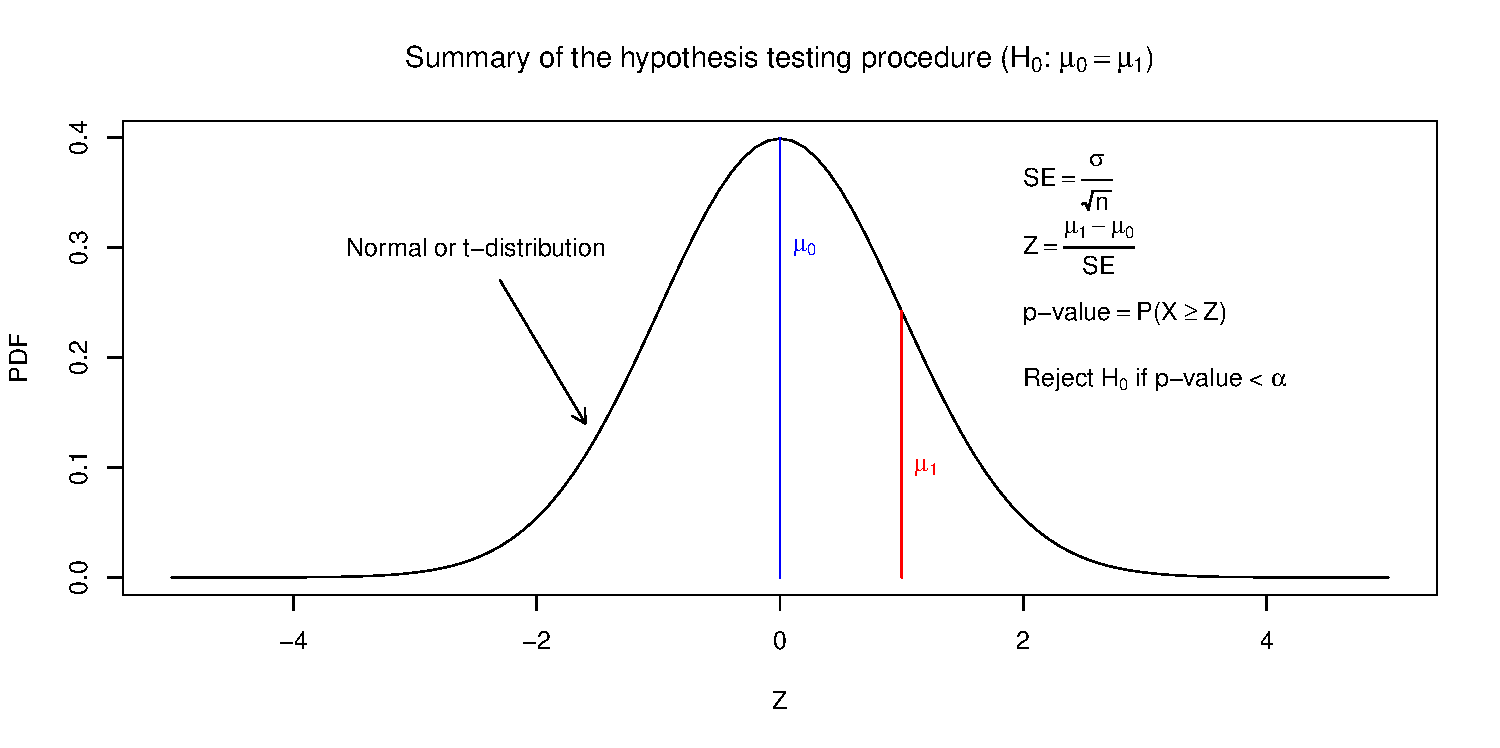
\includegraphics[width=\linewidth]{R/plots/hypothesis_test_summary}
\end{frame}

\begin{frame}{Analysis of Variance (ANOVA)}
    ANOVA, in its simplest form (so-called \emph{one-way ANOVA}), is used to check whether more than two means are equal or not:
    \begin{align*}
        H_0&: \mu_0 = \mu_1 = ... = \mu_n \\
        H_1&: \text{at least one is different}
        \end{align*}

    This can be assessed by analyzing and comparing:
    \begin{itemize}
        \item the variability within groups
        \item the variability between groups
    \end{itemize}
\end{frame}

\begin{frame}[fragile]{ANOVA: Example With 3 Groups}
    Data:
\begin{verbatim}
x <- rnorm(n = 30, mean = 50, sd = 5)
g1 <- x * 1.45 + rnorm(n = length(x), sd = 5)
g2 <- x * 1.50 + rnorm(n = length(x), sd = 5)
g3 <- x * 1.55 + rnorm(n = length(x), sd = 5)\end{verbatim}
    The true means (typically unknown) are: $\bar{\mu}_{g1} = 72.5$, $\bar{\mu}_{g2} = 75$, $\bar{\mu}_{g3} = 77.5$.
    
    The sample means (30 observations in each group) are: $\bar{x}_{g1} = 70.4$, $\bar{x}_{g2} = 72.6$, $\bar{x}_{g3} = 76.3$
    
    Each group could represent e.g. a result of a specific medical treatment. In such case ANOVA can be used to check if there is a difference between 3 treatments.

\end{frame}

\begin{frame}{ANOVA: Example With 3 Groups}
    Are the group means equal?

    \begin{figure}
        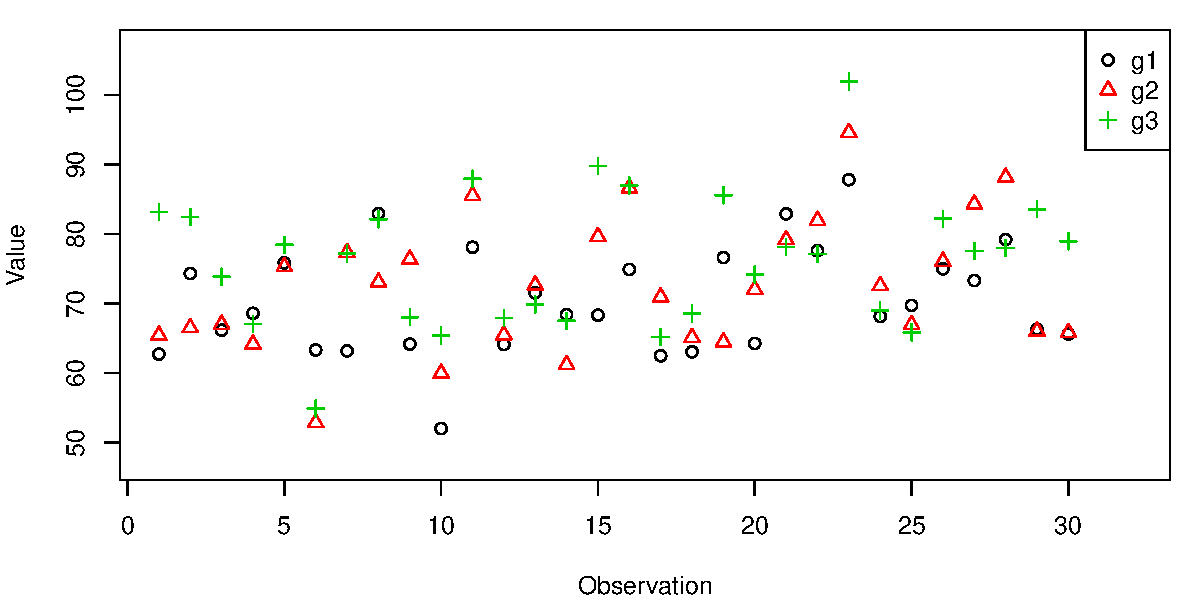
\includegraphics[width=\linewidth]{R/plots/anova_3_groups_scatter}
    \end{figure}
\end{frame}

\begin{frame}{ANOVA: Example With 3 Groups}
    Are the group means equal?

    \begin{figure}
        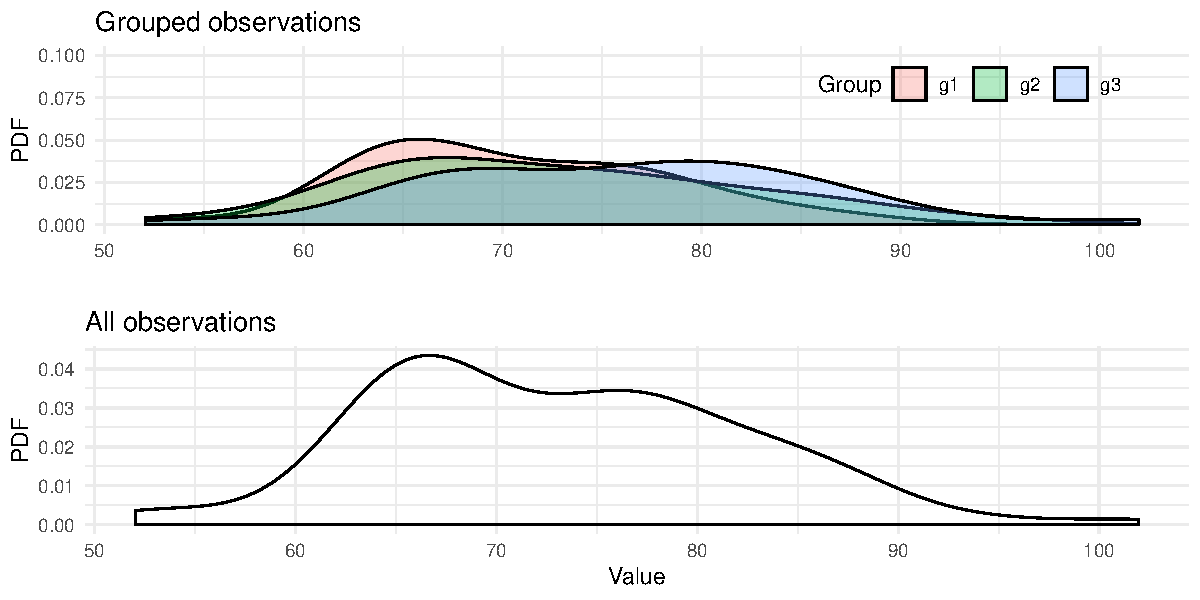
\includegraphics[width=\linewidth]{R/plots/anova_3_groups_density}
    \end{figure}
\end{frame}

\begin{frame}{ANOVA: F-statistic}
    To assess whether the group means are equal,
    we have to compare the \emph{variability between groups}
    with the \emph{variability within groups}.
    \begin{align*}
        F &= \frac{\text{variability between groups}}{\text{variability within groups}}=\\
        &= \frac{\frac{\sum_g (\bar{y}_g - \bar{y})^2}{df_1}}{\frac{\sum_g \sum_i (y_{gi} - \bar{y}_g)^2} {df_2}}
    \end{align*}
    where $y_{gi}$ is the observation $i$ in group $g$, $\bar{y}_g$ is the mean observation in group $g$, $\bar{y}$ is the mean observation in general, $df_1$ and $df_2$ are the respective degrees of freedom.
\end{frame}

\begin{frame}{Variability Between/Within Groups}
    \begin{columns}
        \begin{column}{0.5\textwidth}
            \begin{itemize}
                \item The \textbf{variability betwen groups} describes how far the group means are from one another.
                \item The \textbf{variability within groups} describes how spread the observations are within the groups.
            \end{itemize}
        \end{column}
        \begin{column}{0.5\textwidth}
            \begin{figure}
                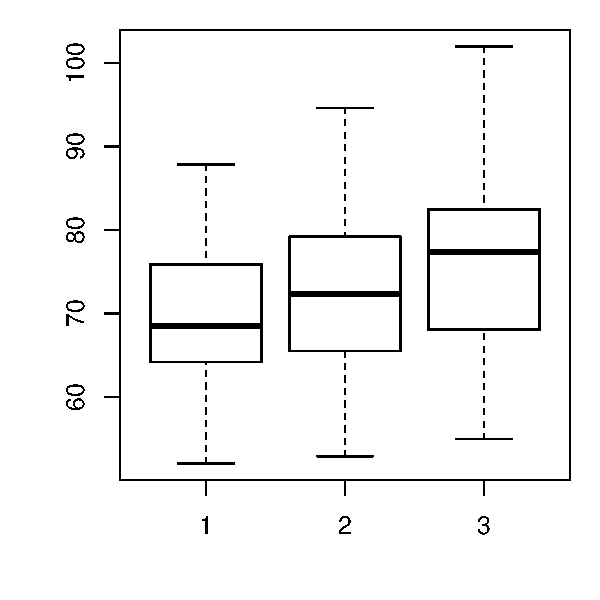
\includegraphics[width=\linewidth]{R/plots/anova_3_groups_boxplot}
            \end{figure}
        \end{column}
    \end{columns}
\end{frame}

\begin{frame}{Degrees of Freedom}
    \begin{itemize}
        \item To be able to compare the variability between and within groups, we need to \emph{normalize the numerator and denominator of $F$}
        \item Both the numerator and denominator represent a sum of squares calculated from different number of elements\\
        ($\sum_g$ vs. $\sum_g \sum_i$)
        \item The degrees of freedom $df$ represents \emph{the number of independent values that the associated term can take on}
        \item For 3 groups, the nominator $df_1 = 3 - 1 = 2$
        \item For 30 observations in each of the 3 groups, the denominator $df_2 = 3 \times 30 - 3 = 87$
    \end{itemize}
\end{frame}

\begin{frame}{ANOVA: Rejecting Null Hypothesis}
    \begin{itemize}
    \item The $F$-statistic is a random variable itself and it follows a special distribution which depends on the degrees of freedom of the numerator ($df_1$) and the denominator ($df_2$).
        
    \item The null hypothesis $H_0: \mu_0 = \mu_1 = ... = \mu_n$ is rejected if $F > F_{critical}$.

    \item $F_{critical}$ is calculated based on the assumed significance level $\alpha$ (typically $0.05$), similarly to the hypothesis testing based on the $t$-distribution.
    \end{itemize}
\end{frame}

\begin{frame}{F-distribution}
    The $F$-distribution depends on the degrees of freedom of the numerator ($df_1$) and the denominator ($df_2$) of the $F$-statistic equation. Exemplary distributions:
    
    \begin{figure}
        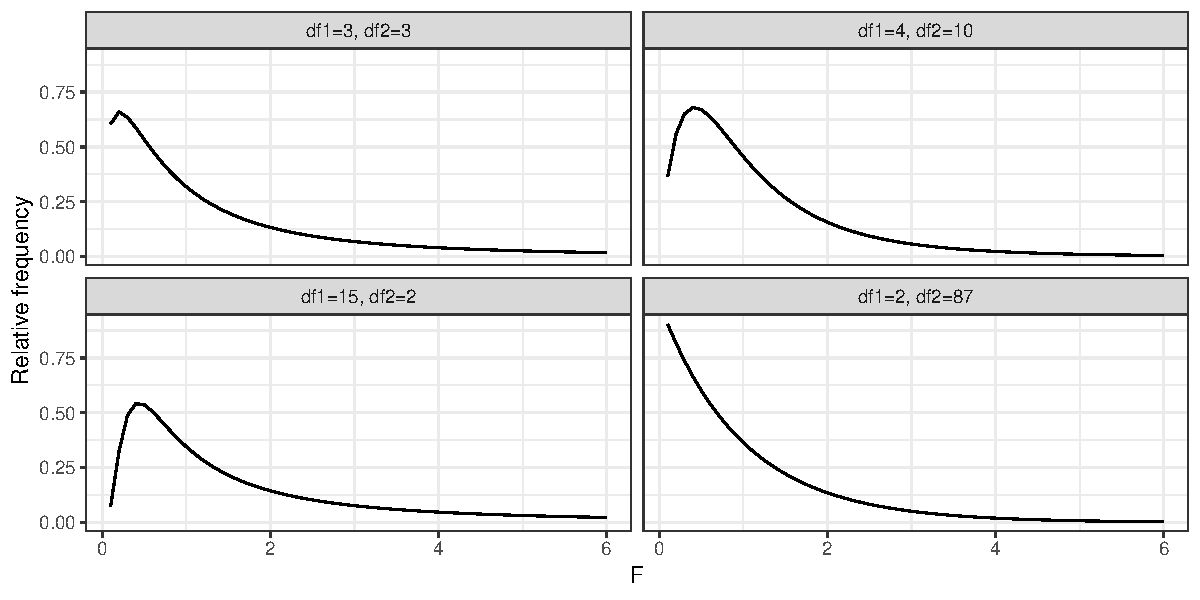
\includegraphics[width=\textwidth]{R/plots/f_distribution}
    \end{figure}
\end{frame}

\begin{frame}[fragile]{ANOVA: Example With 3 Groups}
    ANOVA summary:
    {\small
    \begin{verbatim}
> summary(aov(Value ~ Group, data = df))

            Df Sum Sq Mean Sq F value Pr(>F)  
Group        2    538  269.18   3.324 0.0406 *
Residuals   87   7046   80.99                 
---
Signif. codes:  0 ‘***’ 0.001 ‘**’ 0.01 ‘*’ 0.05 ‘.’ 0.1 ‘ ’ 1
    \end{verbatim}}
    If we assume $\alpha$ equal to 0.05, we can reject $H_0$.\\
    If we assume $\alpha$ equal to 0.01, we cannot reject $H_0$.
\end{frame}